%%%%%%%%%%%%%%%%%%%%%%%%%%%%%%%%%%%%%%%%%%%%%%%%%%%%%%%%%%%%%%%%%%%%%%%%%%%%%
%%%
%%% File: utthesis2.doc, version 2.0jab, February 2002
%%%
%%% Based on: utthesis.doc, version 2.0, January 1995
%%% =============================================
%%% Copyright (c) 1995 by Dinesh Das.  All rights reserved.
%%% This file is free and can be modified or distributed as long as
%%% you meet the following conditions:
%%%
%%% (1) This copyright notice is kept intact on all modified copies.
%%% (2) If you modify this file, you MUST NOT use the original file name.
%%%
%%% This file contains a template that can be used with the package
%%% utthesis.sty and LaTeX2e to produce a thesis that meets the requirements
%%% of the Graduate School of The University of Texas at Austin.
%%%
%%% All of the commands defined by utthesis.sty have default values (see
%%% the file utthesis.sty for these values).  Thus, theoretically, you
%%% don't need to define values for any of them; you can run this file
%%% through LaTeX2e and produce an acceptable thesis, without any text.
%%% However, you probably want to set at least some of the macros (like
%%% \thesisauthor).  In that case, replace "..." with appropriate values,
%%% and uncomment the line (by removing the leading %'s).
%%%
%%%%%%%%%%%%%%%%%%%%%%%%%%%%%%%%%%%%%%%%%%%%%%%%%%%%%%%%%%%%%%%%%%%%%%%%%%%%%

%%%%%%%%%%%%%%%%%%%%%%%%%%%%%%%%%%%%%%%%%%%%%%%%%%%%%%%%%%%%%%%%%%%%%%%%%%%%%
%%%
%%
%% This file, and the corresponding tcdthesis.sty the accompanied it, have
%% been modified for the M.Sc. styles used in Trinity College, Dublin
%%
%%
%%%%%%%%%%%%%%%%%%%%%%%%%%%%%%%%%%%%%%%%%%%%%%%%%%%%%%%%%%%%%%%%%%%%%%%%%%%%%
\documentclass[a4paper, 12pt, oneside]{report}         %% LaTeX2e document.
\usepackage {tcdthesis}              %% Preamble.
\usepackage{graphicx}
\usepackage{cite}
\usepackage{devanagari}
\usepackage[utf8]{inputenc}
\usepackage[english,hindi]{babel}



\mastersthesis                     %% Uncomment one of these; if you don't
% \phdthesis                         %% use either, the default is \phdthesis.

\thesisdraft                       %% Uncomment this if you want a draft
                                     %% version; this will print a timestamp
                                     %% on each page of your thesis.

\leftchapter                       %% Uncomment one of these if you want
%\centerchapter                      %% left-justified, centered or
% \rightchapter                      %% right-justified chapter headings.
                                     %% Chapter headings includes the
                                     %% Contents, Acknowledgments, Lists
                                     %% of Tables and Figures and the Vita.
                                     %% The default is \centerchapter.

% \singlespace                       %% Uncomment one of these if you want
\oneandhalfspace                   %% single-spacing, space-and-a-half
% \doublespace                       %% or double-spacing; the default is
                                     %% \oneandhalfspace, which is the
                                     %% minimum spacing accepted by the
                                     %% Graduate School.

\renewcommand{\thesisauthor}{...}         %% Your official TCD name.
\renewcommand{\thesismonth}{...}                  %% Your month of graduation.
\renewcommand{\thesisyear}{...}                      %% Your year of graduation.
\renewcommand{\thesistitle}{...}            %% The title of your thesis; use mixed-case.
\renewcommand{\thesisauthorpreviousdegrees}{...}  %% Your previous degrees, abbreviated; separate multiple degrees by commas.
\renewcommand{\thesissupervisor}{...}      %% Your thesis supervisor; use mixed-case and don't use any titles or degrees.
% \renewcommand{\thesiscosupervisor}{}                %% Your PhD. thesis co-supervisor; if any.

% \renewcommand{\thesiscommitteemembera}{}
% \renewcommand{\thesiscommitteememberb}{}
% \renewcommand{\thesiscommitteememberc}{}
% \renewcommand{\thesiscommitteememberd}{}
% \renewcommand{\thesiscommitteemembere}{}
% \renewcommand{\thesiscommitteememberf}{}
% \renewcommand{\thesiscommitteememberg}{}
% \renewcommand{\thesiscommitteememberh}{}
% \renewcommand{\thesiscommitteememberi}{}


\renewcommand{\thesisauthoraddress}{...}

\renewcommand{\thesisdedication}{...}     %% Your dedication, if you have one; use "\\" for linebreaks.


%%%%%%%%%%%%%%%%%%%%%%%%%%%%%%%%%%%%%%%%%%%%%%%%%%%%%%%%%%%%%%%%%%%%%%%%%%%%%
%%%
%%% The following commands are all optional, but useful if your requirements
%%% are different from the default values in tcdthesis.sty.  To use them,
%%% simply uncomment (remove the leading %) the line(s).

\renewcommand{\thesisdegree}{Master of Science in Computer Science}  
                                     %% default is "DOCTOR OF PHILOSOPHY"
                                     %% for \phdthesis or "MASTER OF ARTS"
                                     %% for \mastersthesis.  Provide the
                                     %% correct FULL OFFICIAL name of
                                     %% the degree.
\renewcommand{\thesisdegreestream}{ (Data Science)}
                                     %% Default is empty. This is used on
                                     %% the title page of the thesis.

\renewcommand{\thesisdegreeabbreviation}{M.Sc.}
                                     %% Use this if you also use the above
                                     %% command; provide the OFFICIAL
                                     %% abbreviation of your thesis degree.
\renewcommand{\thesistype}{Dissertation}    %% Use this ONLY if your thesis type
                                     %% is NOT "Thesis" for \phdthesis
                                     %% or \mastersthesis.
                                     %% Provide the OFFICIAL type of the
                                     %% thesis; use mixed-case.

% \renewcommand{\thesistypist}{...}  %% Use this to specify the name of
                                     %% the thesis typist if it is anything
                                     %% other than "the author".

%%%
%%%%%%%%%%%%%%%%%%%%%%%%%%%%%%%%%%%%%%%%%%%%%%%%%%%%%%%%%%%%%%%%%%%%%%%%%%%%%



\begin{document}                                  %% BEGIN THE DOCUMENT
\selectlanguage{english}
\thesistitlepage                                  %% Generate the title page.

\thesisdeclarationpage                %% Generate the declaration page.

\thesispermissionpage                 %% Generate the copyright permission page

%\thesisdedicationpage                             %% Generate the dedication page.

\begin{thesisacknowledgments}                     %% Use this to write your
...ACKNOWLEDGMENTS...                          %% acknowledgments; it can be anything
\end{thesisacknowledgments}                       %% allowed in LaTeX2e par-mode.

\begin{thesisabstract}                          %% the abstract for your thesis
...ABSTRACT...
\end{thesisabstract}

\begin{thesissummary}                           %% The summary page for your thesis
...SUMMARY...	
\end{thesissummary}


\tableofcontents                                  %% Generate table of contents.
\listoftables                                     %% Uncomment this to generate list of tables.
\listoffigures                                    %% Uncomment this to generate list of figures.

%%
%% Include thesis chapters here...
%%
  
\chapter{Introduction}
\section{Motivation}
\section{Research Question}
\section{Research Objectives}
To address this research question, five specific research objectives have been defined:
\begin{enumerate}
    \item To create a baseline neural translation model for English to Hindi translation which has the ability to generate above average quality translations by using a large parallel corpus.
    \item To create a new Domain Specific Corpus for the Tourism Domain.
    \item To Fine Tune (Re-Train) the neural translation model by utilizing  a  Hindi Monolingual Corpus.
    \item To Fine Tune (Re-Train) the neural translation model with Domain Specific Training Data.
    \item To Test and Evaluate the neural translation model with Domain Specific Test Data from the Domain Specific Corpus.
\end{enumerate}
\section{Research Challenges}
\section{Overview of Technical Approach}
\section{Dissertation Outline}
\begin{itemize}

\item Chapter 1 provides an introduction to the project. It presents a brief background
and motivation behind the project and then presents the research questions addressed
in this dissertation.
\item Chapter 2 presents the State of the Art of Software Defined Networking and Quality
of Service. This chapter briefly introduces the technologies and areas involved in
this project and then reviews the relevant literature.
\item Chapter 3 explains the architecture and internal details of the various components
of SDN framework that would be used in this project. This chapter sets up the
required technical background for the experiments to follow.
\item  Chapter 4 presents the various experiments conducted in this dissertation. It
presents the statement of the experiment followed by its implementation, results,
and observations.
\item Chapter 5 provides an overview and discussion of the observations gathered throughout
the project. This chapter places the research and findings into the overall big picture of SDN.
\item Chapter 6 concludes the dissertation, talking about the challenges faced and contributions
made in this project. It ends with a discussion on the future work in this direction.
\end{itemize}
	...

  \chapter{State of Art}
In this chapter,the State of the Art in the Machine Translation is discussed. This chapter briefly introduces the technologies and research areas involved in this project and then reviews the relevant literature.

\section{Background}
In 1949, Warren Weaver, a researcher at Rockefeller Foundation, presented a set of proposals for machine based translations which were based on information theory and successes in code breaking during the Second World War(\citeauthor{Weaver},\citeyear{Weaver}).

After few years, the machine translation research began in earnest in many US universities. As described by \cite{Hutchins55thegeorgetown-i.b.m.}, on January 7th 1954, the Georgetown-IBM experiment started, the IBM 701 computer automatically translated 60 Russian sentences into English for the first time in history. This was the first public demonstration of a machine translation system and it garnered much media and public interest.  
 
The ALPAC Report by \cite{Pierce:1966:LMC:1102009} stated that machines cannot compete with the human translation quality and suggested that the funding for Machine Translation should be stopped. But several researchers kept on studying how the machine can be used to create automated language translations. Most of these researches concentrated on limited language pairs with limited input and rule based engines. By the 1980s, a significant number of machine translation engines which relied on mainframe technologies were in use such as SYSTRAN, Logos etc (\citeauthor{wiki:history}, \citeyear{wiki:history}). 

\begin{figure}[h]
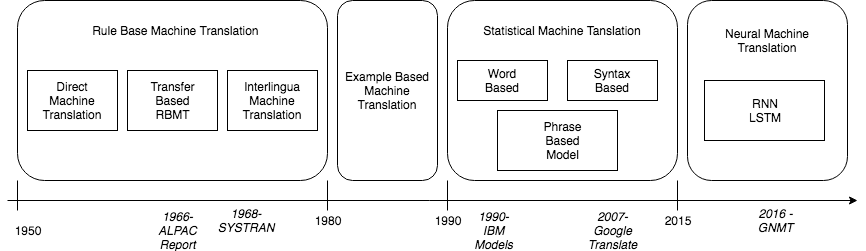
\includegraphics[width=\textwidth,]{figures/timeline.png}
\caption{Timeline of Machine Translation History} \label{sbmt}
\end{figure}

\section{Statistical Machine Translation}

In this section, the evolution of Statistical Machine Translation from Word Based Models to Phrase Based Models and their impact on Machine Translation are discussed in depth as it paves the base of this research.

\subsection{Word Based Translation Models}
\cite{Brown:1988:SAL:991635.991651} proposed the use of statistical methods in Machine Translations. They proposed a translation process where the source text is partitioned into a set of fixed locations, then the glossary is used  to select the set of fixed locations to create a sequence, and finally words in target fixed locations are rearranged to form a target sentence. They successfully developed the statistical techniques for automatic glossary creation and arrangement of target word sequences but failed to provide examples for translated sentences.

\cite{Brown:1990:SAM:92858.92860}   considered only the translation of individual
sentences and used Bayes theorem to implement a new translation model, 
\begin{equation*}
    Pr(S|T)= \frac{Pr (S) Pr (T|S) }{Pr (T) }
\end{equation*}
,where Pr(T$|$S) is the probability the translator produced T in a given target language when  S is a given source language. 

\begin{figure}[h]
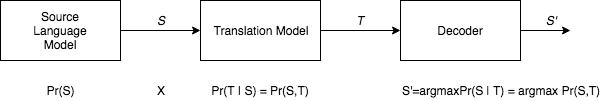
\includegraphics[width=\textwidth]{figures/wbmt.png}
\caption{
A Statistical Machine Translation system  by \cite{Brown:1990:SAM:92858.92860} } \label{wbmt}
\end{figure}

A Source Language Model and a Translation Model outfitted a probability distribution over source-target sentence pair (S,T). The joint probability Pr (S, T) of the combined (S, T) was the result of the probability Pr (S) computed by the language model and the conditional probability Pr (T $|$ S) computed by the translation . The parameters of these models were evaluated automatically from an extensive database of source-target sentence sets utilizing an algorithm which optimized the fit between the models and the information.

They experimented their model by creating an English vocabulary with 9,000 most common English words from Canadian Hansard data\footnote{\url{https://www.lipad.ca/},accessed:10.08.2018}, and the French vocabulary with 9,000 most common French word. They applied their iterative algorithm to estimate some 81 million parameters from 40,000 pairs of sentences in each of the language. In the second approach, they used the statistical approach to decode 73 new french sentences. If the decoded sentence exactly matched the original translation it was assigned \textit{exact} category, otherwise it was assigned \textit{alternate} or \textit{different} or \textit{wrong} or \textit{ungrammatical} based on the quality of translation.The system performed affirmatively for 48\% of the cases.

\cite{Brown:1993:MSM:972470.972474} described a series of five statistical models for the translation process and gave algorithms for estimating the parameters of these models given a set of bilingual pairs of sentences. These models were later considered as the IBM alignment models. They defined the concept of word-by-word alignment between the pair of bilingual sentences. Their algorithm assigned a probability to each of these word-by-word alignments for any given pair of sentences. Though their research was confined to smaller English and French translations but it was a considerable improvement to the the alignment of word-by-word relationships in the pair of sentences.

\cite{Vogel:1996:HWA:993268.993313} described a new model for word alignment in the Statistical Machine Translation using first-order Hidden Markov Model(\citeauthor{Jelinek76continuousspeech}, \citeyear{Jelinek76continuousspeech}) as it solved the time alignment problem for speech recognition. The main idea behind the model was to make the word-by-word alignment probabilities depend on the alignment positions rather than the absolute positions. The HMM-based model produced translation probabilities on par with the mixture alignment model and position alignments were much smoother in HMM-based model.

\cite{Och:1999:EMD:977035.977046} described a method to determine bilingual word classes to be used in Statistical Machine Translation. They developed an optimization criterion based on the maximum likelihood approach and further described a clustering algorithm. The results of their experiments showed that the usage of bilingual word classes improved the statistical machine translations significantly.

The IBM models were implemented in a toolkit called GIZA by \cite{Giza}, later updated to GIZA++ by \cite{Och:2000}.GIZA++ is open source and widely used.

\subsection{Syntax Based Translation}
A syntax-based statistical translation model was proposed by \cite{Yamada:2001:SST:1073012.1073079}. Their model transformed a source-language parse tree into a target-language string by applying stochastic operations at each node. Those operations captured the linguistic differences such as word order and case marking. The model produced word alignments which were better those produced by IBM Model 5 (\citeauthor{Brown:1993:MSM:972470.972474}, \citeyear{Brown:1993:MSM:972470.972474}). 

They assumed that an English parse three $\varepsilon$  is transformed into a French sentence $f$. The English parse tree $\varepsilon$ consisted of nodes $\varepsilon_1$,$\varepsilon_2$,.. $\varepsilon_n$ and the French sentence consisted of French words $f_1,f_2,..,f_m$.
The authors considered three random variables, N, R, and T as channel operations which were applied to each node. \textit{Insertion} N is an operation that inserts a French word just before or after the node and it can be either none, left or right. \textit{Reorder} R is an operation that is used to change the order of the children of the node. \textit{Translation} T is an operation which translates a terminal English leaf word into a French word. 

The notation $ \theta = ( v, p,t )$  represents a  set of values of $N_i$, $R_i$ , T. Whereas, $ \theta_i = ( v_i, p_i,t_i )$  is a set of values of random variables associated with $\varepsilon_i$. $ \theta = \theta_1,\theta_2,...,\theta_n$is the set of all random variables associated with a parse tree $\varepsilon$ = $\varepsilon_1$,$\varepsilon_2$,..., $\varepsilon_n$.

 The probability of getting a French sentence $f$ given an English parse tree $\varepsilon$ is given by,
 
 \begin{equation}
     p(f|\varepsilon)=\sum_{\theta:Str(\theta(\epsilon))=f}p(\theta|\varepsilon)
 \end{equation}
as described by \cite{Yamada:2001:SST:1073012.1073079}.

For the estimation of the model parameters they used the EM algorithm (\citeauthor{10.2307/2984875}, \citeyear{10.2307/2984875}) which automatically updates the model parameters to maximize the likelihood of the training corpus. Initially the model parameters were initialized and afterwards for each and every iteration, the number of events were counted and weighted by the probabilities of the event. Before the next iteration, the current model parameters were used to calculate the probabilities of the events and then the model parameters were re-estimated using the counts.

For the experiments they trained their model on a small English $\rightarrow$ Japanese corpus and evaluated the performance of their model along with IBM Model 5. To evaluate performance they let the models generate the most probable alignment of the training corpus (called the Viterbi alignment) which shows  how the learned model induced the internal structure of training data.
The alignment produced by their model and IBM Model 5 are shown in Figure (\ref{sbmt}) , where the darker lines represent the alignments judged accurate by humans. They further obtained average score of the first 50 sentence
pairs in the corpus and counted the number of perfectly aligned sentences, which is shown in Table \ref{sbmtt}.Their model got a much better result than IBM Model 5 with more number perfectly aligned sentences.
\begin{figure}
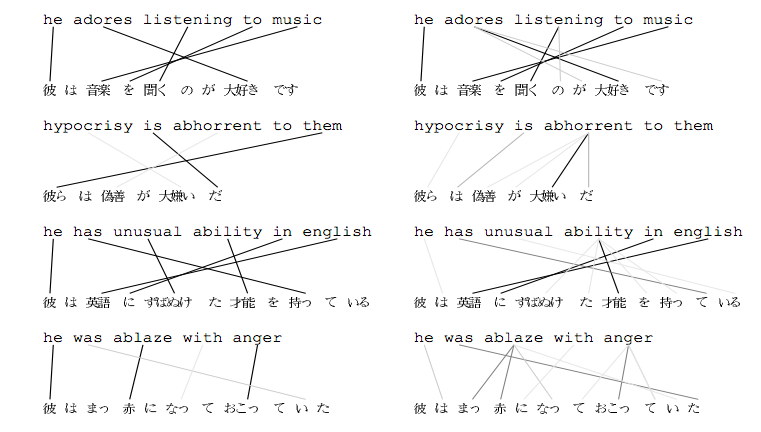
\includegraphics[width=\textwidth,,height=250pt]{figures/syntax1.png}
\caption{Viterbi Alignments: \cite{Yamada:2001:SST:1073012.1073079}'s model (left) and IBM Model 5 (right). Darker lines are judged more
correct by humans.} \label{sbmt}
\end{figure}

\begin{table}[h]
\centering
\begin{tabular}{ |c|c|c| } 
 \hline & Alignment ave. score & Perfect sents \\ 
 \hline \cite{Yamada:2001:SST:1073012.1073079}'s Model & 0.582 & 10 \\ 
 \hline IBM Model 5 & 0.431 & 0 \\ 
 \hline
\end{tabular}
\caption{Human Evaluation : \cite{Yamada:2001:SST:1073012.1073079}'s model and IBM Model 5.}\label{sbmtt}
\end{table}


\subsection{Phrase Based Translation Model}
Over the years many researchers tried to improve the quality of machine translations by using Phrase Based Translation Model. The align template model by \cite{W99-0604} can be considered as the initiation towards phrase based models. A method similar to Phrase Based Translation was used in a Syntax Based Translation system by \cite{Yamada:2001:SST:1073012.1073079} which has been discussed earlier. A joint-probability model for phrase translation was introduced by \cite{Marcu:2002:PJP:1118693.1118711} and achieved more accurate translations than those produced using IBM Model 4.

A novel phrase-based translation model and decoding algorithm was proposed by \cite{Koehn:2003:SPT:1073445.1073462} which enabled them to evaluate and compare several previously proposed phrase-based translation models. They designed an uniform framework to compare different other translation models. The model proposed by \cite{Koehn:2003:SPT:1073445.1073462} was based on the noisy channel model(\cite{Brown:1993:MSM:972470.972474}) and they used the Bayes rule to reformulate the translation probability for translating a foreign sentence $f$ into English $e$ as

$$
argmax_ep(e|f)= argmax_ep(f|e)p(e)
$$

That allowed for language model $p(e)$ and a separate translation model $p(f|e)$.

During the decoding phase, the foreign input sentence $f$ was segmented into a sequence of $I$ phrases $\bar{f_1^1}$ . Uniform probability distribution over all possible segmentation were assumed by the authors. Each foreign phrase $\bar{f_i}$ in $\bar{f_1^1}$ was translated into an English phrase $\bar{e_i}$, though there were reordering of the English sentences. A probability distribution $\phi(\bar{f_i}|\bar{e_i})$ modeled the entire phrase translation and due to the Bayes Rule, the direction of translation is inverted from a modeling standpoint. 

Reordering of the English output phrases was modeled by a relative distortion probability distribution $d(a_i$ - $b_{i-1})$, where the start position of the foreign phrase that was translated to the English phrase was denoted by $a_i$ and the end position of the foreign phrase was denoted by $b_{i-1}$. Throughout their experiments, they trained the distortion probability distribution $d (.)$ using a joint probability model. Further to optimize the performance of the model , they introduced a factor $w$ for each generated English word in addition to trigram language model $p_{LM}$. 

The best English output sentence $e_{best}$ given a foreign input sentence $f$ according to their model is ,

$$
 e_{best}= argmax_ep(e|f)
         = argmax_ep(e|f)
$$

The phrase-based decoder developed by \cite{Koehn:2003:SPT:1073445.1073462} employed a beam search algorithm similar to the one by \citep{Jelinek76continuousspeech}  for the comparison of different phrase-based translation models.

Their results showed that phrase based translation gave better performance than the word based models by using lexical weighting of phrases and a phrase extraction heuristic.

\subsection{Hierarchical Phrase-Based Translation Model}

\cite{Chiang:2005:HPM:1219840.1219873} presented a  phrase-based machine translation model that used hierarchical phrases – phrases that contained subphrases. The basic phrase-based model was an instance of the noisy-channel approach by \cite{Brown:1993:MSM:972470.972474}, the other variations such as (\citeauthor{W99-0604}, \citeyear{W99-0604}; \citeauthor{Koehn:2003:SPT:1073445.1073462}, \citeyear{Koehn:2003:SPT:1073445.1073462}) had a distortion model that reordered phrases independently. The authors felt that there was a need of technique which capture translations whose scope was larger than few consecutive words, specifically in complex languages like Mandarin. The phrase-based translation worked well with phrase reordering but failed to accomplish inversion of two phrases within a complex sentence. They proposed the use of hierarchical phrases which consisted of both words and sub-phrases to address this problem. Their model was based on a weighted synchronous Context Free Grammar ( \citeauthor{Aho:1969:SDT:1739930.1740037}, \citeyear{Aho:1969:SDT:1739930.1740037}). The model built partial translations using the hierarchical phrases and then combined them serially in a standard phrase-based model.  Instead of using the traditional noisy-channel approach , they used a more general log-liner model as proposed by \cite{Och:2002:DTM:1073083.1073133}.

They evaluated their model on a Mandarin $\rightarrow$ English translation task and compared their model against Pharaoh (\citeauthor{10.1007/978-3-540-30194-3_13}, \citeyear{10.1007/978-3-540-30194-3_13}). Their experiments showed that hierarchical phrase pairs can be learned by the models without using any syntactically-annotated training data and can improve the translation accuracy significantly compared to the phrase-based systems. Though the hierarchical models encouraged the consolidation of syntactic information but failed to provide a statistically significant gain.

\begin{table}[h]
\centering
\begin{tabular}{ |c|c| } 
 \hline System & BLEU  \\
 \hline
 Pharaoh & 0.2676  \\ 
 hierarchical & 0.2877 \\ 
  hierarchical+constituent & 0.2881 \\ 
 \hline
\end{tabular}
\caption{Results on baseline system and hierarchical system. \cite{Chiang:2005:HPM:1219840.1219873}}\label{hbmtt}
\end{table}

\subsection{Moses and Factored Translation Model}
Moses is an open-source implementation of the statistical machine translation developed by \cite{Koehn:2007:MOS:1557769.1557821}. The Statistical Machine Translation Systems are trained on huge quantities of parallel bilingual data and larger quantities of monolingual data. The parallel data is collection of sentences in two different languages which is sentence aligned, that is the sentence in one language is matched with the sentence in corresponding language. In Moses, the system takes parallel data for the training process and uses the co-occurrences of phrases to infer translation correspondences between two languages of interest. In phrase-based machine translation, these correspondences are essentially between ceaseless arrangements of words, whereas in hierarchical phrase-based machine translation or syntax-based translation, more structure is added to the correspondences. Apart from being an open-source toolkit for SMT, Moses extended the phrase based translation with factors and confusion network decoding. The Phrase Based Model in Statistical Machine Translation was limited to the mapping of small text chunks with no express utilization of etymological data, be it morphological, syntactic, 
or on the other hand semantic. Previous researches showed that these additional sources of information are valuable when integrated into pre-processing or post-processing steps. Moses also integrated confusion network decoding, a mechanism which allowed translation of ambiguous input and enabled tighter integration of speech recognition and machine translation. The machine translation system examines a network of different word choices instead of passing along the one-best output of the recognizer. 
\subsubsection{Factored Translation Model}
The non-factored SMT such as phrase based SMT typically dealt only with surface form of words and had one phrase table as shown in Figure \ref{nofac}. 
\begin{figure}
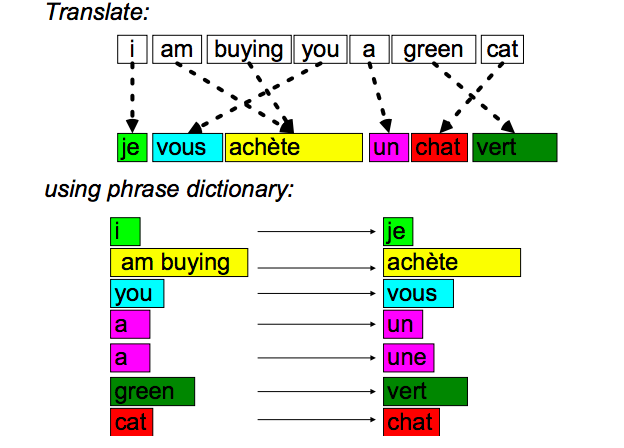
\includegraphics[width=\textwidth,,height=250pt]{figures/moses1.png}
\caption{Non-factored Translation. \citep{Koehn:2007:MOS:1557769.1557821}} \label{nofac}
\end{figure}

In factored translation model, the surface forms may be augmented with different factors, such as POS tags or lemma. This created a factored representation of each word, refer Figure \ref{factrans}.
\begin{figure}
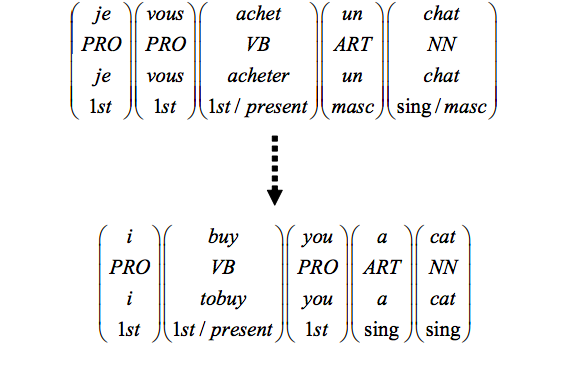
\includegraphics[width=\textwidth,height=250pt]{figures/moses2.png}
\caption{Factored Translation. \citep{Koehn:2007:MOS:1557769.1557821}} \label{factrans}
\end{figure}

The authors suggested that mapping of source phrases to target phrases might be decomposed into a few stages. Decomposition of the decoding process into different steps implied that diverse components can be modelled independently. Modelling factors in isolation takes into consideration adaptability in their application. It can likewise increment accuracy and decrease sparsity by limiting the number conditions for each step. For example, a surface form can be decomposed to surface forms and lemma, as shown in Figure \ref{exfac}.
\begin{figure}
\begin{center}
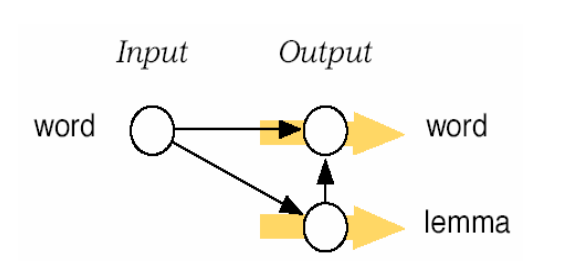
\includegraphics[width=300pt]{figures/moses3.png}
\caption{Example of graph of decoding systems. \citep{Koehn:2007:MOS:1557769.1557821}} \label{exfac}
\end{center}
\end{figure}

The graph was allowed to be user definable, thus it provided a scope for experimentation with different configurations to find the optimum configuration for the given language pair and data. The authors considered the factors on the source sentence to be fixed, therefore they did not implement any decoding step to create source factors from other source factors. They designed Moses as such becuase every factor on the target language could have its own language model.  Many factors such as lemmas and POS tags are sparser than surface forms so it was possible to create a higher order language models for these factors.

\subsubsection{Confusion Network Decoding}
The authors wanted to meet the increasing demands of integrating machine translation technology into bigger information processing systems with upstream NLP/speech processing tools such as named entity recognizers, speech recognizers, morphological analyzers, etc. The authors experimented with confusion networks by focusing on the speech translation case, where initially the input is generated by a speech recognition system. Their immediate goal was to improve the language translation by combining the speech recognition and machine translation models. The biggest problem in translation of spoken language was, its proneness to speech recognition errors which used to corrupt the input syntax and its meaning. Previous researches also showed that better translations can be obtained from the transcriptions of the speech recognizer.  The authors found that significant improvements could have been achieved by applying machine translation techniques on larger sets of transcription texts generated by the speech recognizers and combining the scores of acoustic models, language models, and translation models. 

In Moses, they implemented the confusing network decoding as discussed in \citep{4218346}, and they developed a simpler translation model and a more efficient implementation of the search algorithm.

\subsection{Challenges in SMT}

Statistical Machine Translation generated translation using statistical models whose parameters are derived from the analysis of bilingual text corpora. 

There were several challenges faced in statistical machine translation, which are as follows\citep{wiki:smt}:

\begin{itemize}
    \item \textbf{Lack of Large Parallel Corpora}   Statistical Machine Translation systems need large sets of parallel data for the translation task. But the unavailability of large corpora in low resource language posed a challenge to the SMT and it affected the efficiency of translation models in several low resource languages.
    \item\textbf{Sentence Alignment }   In parallel corpora, a single sentence in one language when translated into other language may be more than one sentence, thus aligning such sentences in parallel becomes a challenge. Further, algorithms such as Gale-Church alignment algorithm needed to be used for sentence alignment(\citeauthor{Gale:1991:PAS:981344.981367},\citeyear{Gale:1991:PAS:981344.981367}).
     \item\textbf{Word Alignment }      Most of the popular parallel corpora is sentence aligned or sentence alignment can be done using the previously mentioned Gale-Church Algorithm(\citeauthor{Gale:1991:PAS:981344.981367},\citeyear{Gale:1991:PAS:981344.981367}). The real challenge lies for word alignment, to know which word in source language aligns with which word in the target language, though IBM models and HMM-approach(\citeauthor{Vogel:1996:HWA:993268.993313},\citeyear{Vogel:1996:HWA:993268.993313} provides a better solution to this problem. 
     \item\textbf{Statistical anomalies }  Sometimes the real-world training sets tends to overwrite the translations of proper nouns. An abundance of particular noun in the training set may tend overwrite a less frequent noun in translated sentence. An example would be like,"\textit{Thóg mé an eitilt go Ibiza} " in Irish should ideally translate to "\textit{I took the flight to Ibiza}" in English, but gets to "\textit{I took the  flight to London"} due to abundance of "\textit{flight to London}" in the training data.
     \item\textbf{Idioms }Depending upon the corpora utilized for the translation task, idioms may not translate "idiomatically". For instance, utilizing Canadian Hansard [Reference] as the bilingual corpus, "hear" may constantly be meant "Bravo!" since in Parliament "Hear, Hear!" moves toward becoming "Bravo!". 
     \item\textbf{Different Word Orders}    Different languages follow different word orders. In some languages, classification can be done by naming the typical order of subject (S), verb (V) and Object (O) in a sentence and in some languages, it can be represented as SVO or VSO. An example, the English sentence \textit{“Tom is eating vegetables”} is having the SVO word order, where as its translation in Hindi can be either \textit{“Tom vegetables kha raha hai”} which is SOV or \textit{“Vegetables kha raha hai Tom”} which is of the OVS order. 
     \item\textbf{Out of vocabulary (OOV) words}    The SMT systems typically stores the different words and their word forms as separate symbols in their vocabulary. The unrelated words or the phrases which are not part of the training data can not be translated. This is generally due to the lack of training data, changes in the human domain or some morphological differences. 
     \item\textbf{Mobile devices}   The rapid increase in the processing power of tablets and cell phones, combined with the wide accessibility of machine translation systems. However, when speech recognition system are comnined with SMT for portable devices it raises several lexical issues which deteriorate the quality of translations.
     
\end{itemize}
\section{Neural Machine Translation}
\subsection{Background}

In 2013, a new end-to-end encoder-decoder structure for machine translation was proposed by \cite{D13-1176}. They introduced a class of probabilistic continuous translation models called Recurrent Continuous Translation Models which were purely based on continuous representations for words, phrases and sentences and did not rely on alignments or phrasal translation units.

\cite{NIPS2014_5346} proposed the use of Deep Neural Networks in Sequence to Sequence learning for Machine Translations. Their method used a multi-layered Long Short-Term Memory (LSTM) to map the input sequence to a vector of a fixed dimensions, and then used another deep LSTM to decode the
target sequence from the vector. Their results showed that Neural Machine Translation system having large deep LSTM with a limited vocabulary can outperform a standard SMT-based system. 

\begin{figure}[h]
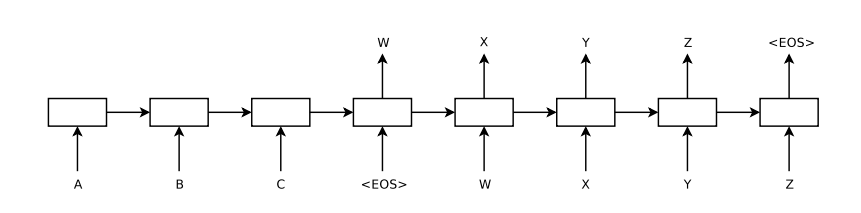
\includegraphics[width=\textwidth]{figures/nmt1.png}
\caption{ The basic architecture Neural Machine Translation system by \cite{NIPS2014_5346} } \label{gnmt1}
\end{figure}

\cite{DBLP:journals/corr/ChoMGBSB14} proposed a new neural network model with two recurrent neural networks (RNN) as Encoder and Decoder. One RNN encoded a sequence of symbols into a fixed length vector representation, while the other decoded the representation into another sequence of symbols. Their results showed that RNN Encoder–Decoder were able to capture both semantic and syntactic structures of the phrases.

\cite{DBLP:journals/corr/BahdanauCB14} proposed a method which allowed a model to automatically soft-search for parts of a source sentence that are relevant in predicting a target word,without having to form these parts as a hard segment explicitly. With this approach, they achieved e a translation performance comparable to the existing state-of-the-art
phrase-based system on the task of English-to-French translation.

\cite{DBLP:journals/corr/LuongPM15} proposed two effective classes of attentional mechanism, a global approach which always attends to all source words and a local one that only looks at a subset of source words at a time.Their ensemble model using different attention architectures established a new state-of-the-art result in the WMT'15 English to German translation task with 25.9 BLEU points.

\cite{DBLP:journals/corr/JozefowiczVSSW16} experimented with different neural network models on different sizes of corpora, their experiments showed that RNNs can be trained
on large amounts of data, and they outperform competing models
including carefully tuned N-grams. Their experiments showed that a large, regularized LSTM LM, with projection layers and trained with an approximation to the true Softmax with importance sampling performed much better than N-grams.


In the Findings of First Conference on Machine Translation (WMT'16), the neural machine translation systems that participated in the WMT evaluation outperformed phrase-based statistical machine translation system by up to 3 BLEU score (\citeauthor{WMT:2016}, \citeyear{WMT:2016}).

\cite{koehnblog} wrote, \textit{"Neural Machine Translation (NMT) is an exciting and promising new approach to Machine Translation. However, while the technology is promising we still have some way to go to commercial implementations that can rival Rule Based Machine Translation (RBMT) and Statistical Machine Translation (SMT) in all use cases. Some recent claims by industry players to suggest that near human quality is right around the corner for all of us, might be a bit of an over-simplification."}. He argued that even if the Neural Machine Translation systems produce superior quality results, its very difficult to implement such systems at an industrial scale as it would require huge investment in infrastructure for processing the translations.

\subsection{Google's Neural Machine Translation}
\cite{45610} proposed a model (see Figure \ref{gnmt1}) which follows the common sequence-to-sequence learning framework \citep{NIPS2014_5346} with attention \citep{DBLP:journals/corr/BahdanauCB14}. The model has three components: an encoder network, a decoder network and an attention network. The encoder network converts a source sentence into a list of vectors, one vector per input symbol. When this list of vectors is passed to decoder network it produces one symbol at a time until it encounters the special end-of-sentence symbol (EOS). The encoder and decoder are connected through an attention module which allows the decoder to focus on different regions of the source sentence during the course of decoding. 
\begin{figure}[h]
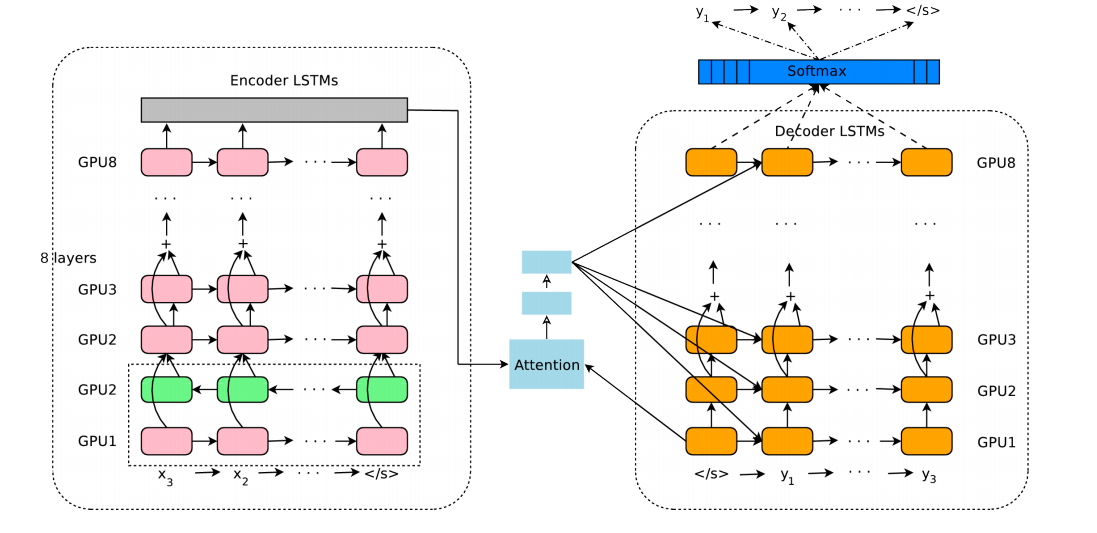
\includegraphics[width=\textwidth]{figures/gnmt1.png}
\caption{ The model architecture of GNMT, Google’s Neural Machine Translation system \citep{45610}. } \label{gnmt1}
\end{figure}

Figure \ref{gnmt1} shows the architecture of the Google Neural Translation Model, \cite{45610}'s description of the architecture is as follows. On the left is the encoder network, on the right is the decoder network, in the middle is the attention module. The bottom encoder layer is bi-directional: the pink nodes gather information from left to right while the green nodes gather information from right to left. The other layers of the encoder are uni-directional. Residual connections start from the layer third from the bottom in the encoder and decoder. The model is partitioned into multiple GPUs to speed up training. In their setup, they have 8 encoder LSTM layers (1 bi-directional layer and 7 uni-directional layers), and 8 decoder layers. With this setting, one model replica is partitioned 8-ways and is placed on 8 different GPUs typically belonging to one host machine. During training, the bottom bi-directional encoder layers compute in parallel first. Once both finish, the uni-directional encoder layers start computing, each on a separate GPU. To retain as much parallelism as possible during running the decoder layers, they used the bottom decoder layer output only for obtaining recurrent attention context,which is sent directly to all the remaining decoder layers. The softmax layer is also partitioned and placed on multiple GPUs. Depending on the output vocabulary size they either have them run on the same GPUs as the
encoder and decoder networks, or have them run on a separate set of dedicated GPUs.

They assumed (X,Y) as a source and target sentence pair , and $X$ = $x_1,x_2,x_3,..,x_M$ as the sequence of M symbols in the source text and $Y$= $y_1,y_2,y_3,.., y_N$ as the sequence of $N$ symbols in target text. The encoder is a simple function of the following form:
$$x_1,x_2,..,x_M = EncoderRNN(x_1,x_2,..,x_M)$$

Their decoder network is implemented as an amalgamation of an RNN network and a softmax Layer. The decoder RNN network creates a hidden state $Y_i$ for the next symbol to be predicted, which then goes through the softmax layer to generate a probability distribution over candidate output symbols. In their experiments the authors found out that Neural Machine Translation systems must have deep RNNs for encoder and decoder networks to achieve good accuracy, they need to capture the minute irregularities in the source and target languages. 

The Attention Model they implemented in their research is similar to \citep{DBLP:journals/corr/BahdanauCB14}. More precisely, they assumed $y_{i-1}$ to be the decoder RNN from the previous decoding step which is the bottom decoder layer. Attention context $a_i$ , for the current time step is computed according to the following formulas:

\begin{align*}
    s_t &= AttentionFunction(y_{i-1},x_t)\;\forall t \;1\leq t\leq M\\
    p_t &= \frac{exp(s_t)}{\sum_{t=1}^M exp(s_t)}\;\forall t \;1\leq M\\
    a_i &= \sum_{t=1}^M exp(s_t) p_t.x_t
\end{align*}


Where \textit{AttentionFunction} in their implementation is a feed forward network with one hidden layer\citep{45610}.

The authors acknowledged the fact that simply tacking up more Layers of LSTM makes the network slower and difficult to train, likely due to exploding and vanishing gradient problems \citep{DBLP:journals/corr/NorouziBCJSWS16,Hochreiter01gradientflow}. The simple stacked LSTM layers worked well up to 4 to 6 layers but performed very poorly beyond 8 layers. 

\begin{figure}
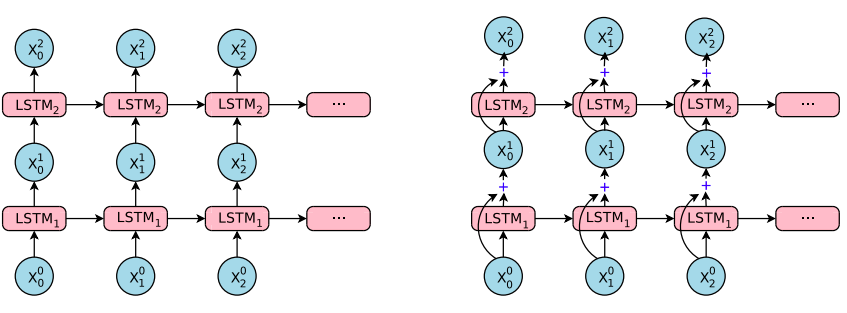
\includegraphics[width=\textwidth]{figures/gnmt2.png}
\caption{The difference between normal stacked LSTM and their stacked LSTM with residual connections \citep{45610}.} \label{gnmt2}
\end{figure}

The authors were motivated by the idea of modelling differences between an intermediate layer’s output and the targets, which has shown to work well for many projects in the past \citep{NIPS1989_207,7780459,DBLP:journals/corr/SrivastavaGS15}, they introduced residual connections among the LSTM layers in a stack (See Figure \ref{gnmt2}). Residual Connection greatly improved the gradient flow in the backward pass, which allowed them to train their encoder and decoder networks with 8 LSTM layers. In translation systems, the information required to translate some words in the output language can appear anywhere in the source language. They decided to use a bi-directional RNN for the encoder to have the optimum scenario in the encoder network (See Figure \ref{gnmt3}). They used the bi-directional connections for the bottom encoder layer while keeping other layer uni-directional to allow maximum parallelization during computation. 

\begin{figure}
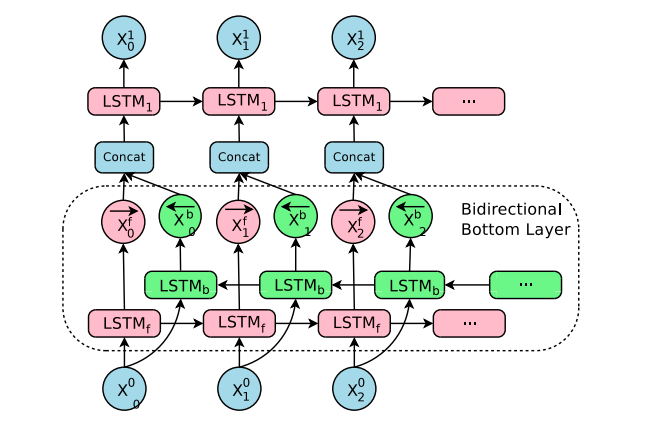
\includegraphics[width=\textwidth,height=250pt]{figures/gnmt3.png}
\caption{Residual connections in Google NMT \citep{45610}} \label
{gnmt3}\end{figure}

Due to the complexity of their model the authors implemented model parallelism and data parallelism to speed up the training. But Model Parallelism came up with certain constraints on their Model Architecture like they could not bi-directional LSTM layers for their all encoder layers.  The authors implemented the Wordpiece model which was initially developed by Google Speech Recognition System \citep{conf/icassp/SchusterN12} for solving Japanese/ Korean segmentation problem to solve the out-of-vocabulary translation problems. 


\begin{figure}
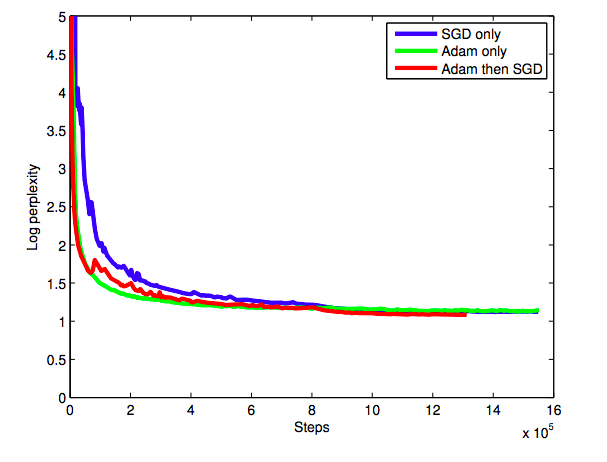
\includegraphics[width=\textwidth,height=250pt]{figures/gnmt5.png}
\caption{Log perplexity vs. steps for Adam, SGD and Adam-then-SGD on WMT En $\rightarrow$ Fr during maximum
likelihood training \citep{45610}.} \label{fig1}
\end{figure}

The authors used two publicly available corpora WMT’14\footnote{\url{http://www.statmt.org/wmt14/}} English-to-French (WMT En $\rightarrow$Fr) and English-to-German (WMT En $\rightarrow$De) as benchmarks for their Neural Machine Translation systems. In addition to these publicly available corpora they used Google’s translation production corpora which is much bigger than the WMT corpora for a given language pair. The WMT En$\rightarrow$Fr contains 36M sentence pairs while the En$\rightarrow$De contains 5M sentence pairs. They evaluated their models by carrying out side by side Human evaluations along with standard BLEU score metric. The side by side scores ranged from 0 to 6, with a score of 0 meaning “completely nonsense translation”, and a score of 6 meaning “perfect translation: the meaning of the translation is completely consistent with the source, and the grammar is correct”. They trained the models using the system they implemented in TensorFlow. For the initial stage of maximum likelihood training they used a combination of Adam \citep{DBLP:journals/corr/KingmaB14} and SGD learning algorithms provided by TensorFlow. They ran Adam for the first 60K steps , after which they switched to simple SGD. They found that in the beginning Adam accelerates training but Adam alone converged to a worse point than a combination of Adam first, followed by SGD ( Figure 2.5). For the Adam part they used a learning rate of 0.0002 and for the SGD part they used a learning rate of 0.5. They used word-based, character-based, mixed-character-based and several wordpiece models with different vocabulary sizes for the experiments. Table summarizes the results they achieved on WMT En $\rightarrow$ Fr dataset. Their best model, WPM-32K achieved a BLEU score of 38.95. The WMT En $\rightarrow$ De was much more difficult than the En $\rightarrow$ Fr due to the less size of training data and German is a more morphologically rich language which needs vocabulary for word models. Their best model WPM-32K achieved a BLEU score of 24.61. 

\begin{table}[h!]
\centering
 \begin{tabular}{ |ccc| } 
  \hline Model & BLEU &  CPU decoding time
 (s) \\ 
  \hline  Word &  37.90 & 0.2226\\
  Character (512 nodes)& 38.01 & 1.0530\\
  WPM-8K & 38.27 &  0.1919\\
  WPM-16K &  37.60 & 0.1874\\
  WPM-32K & 38.95 &  0.2118\\
  Mixed Word/Character & 38.39 &  0.2774\\
  \hline PBMT \citep{durrani} & 37.0 &\\
  LSTM (6 layers)\citep{DBLP:journals/corr/LuongSLVZ14}  &  31.5 & \\
  LSTM (6 layers + PosUnk) \citep{DBLP:journals/corr/LuongSLVZ14} &33.1&\\
  Deep-Att \citep{DBLP:journals/corr/ZhouCWLX16} &  37.7&\\
  Deep-Att + PosUnk \citep{DBLP:journals/corr/ZhouCWLX16} &39.2&\\
  \hline
 \end{tabular}
\caption{Results of the Single model on WMT En$\rightarrow$ Fr \citep{45610}}
\end{table}

\begin{table}[h!]
\centering
 \begin{tabular}{ |ccc| } 
  \hline Model & BLEU &  CPU decoding time
 (s) \\ 
  \hline  Word &  23.12 & 0.2972\\
  Character (512 nodes)& 22.62 & 0.8011\\
  WPM-8K & 23.50 &  0.2079\\
  WPM-16K & 24.36 & 0.1931\\
  WPM-32K & 24.61 & 0.1882\\
  Mixed Word/Character & 24.17 & 0.3268\\
  \hline PBMT \citep{durrani} & 20.7 &\\
  RNNSearch \citep{DBLP:journals/corr/LuongSLVZ14}  &  16.5 & \\
  RNNSearch-LV \citep{DBLP:journals/corr/LuongSLVZ14} &16.9&\\
  Deep-Att \citep{DBLP:journals/corr/ZhouCWLX16}& 20.6&\\
  \hline
 \end{tabular}
\caption{Results of the Single model on WMT En$\rightarrow$ De \citep{45610}}
\end{table}


They further used RL training to fine-tune the sentence BLEU score after normal maximum-likelihood training. The results of the best models showed that the fine-tuning of the models with RL can improve the BLEU scores. 


\begin{table}[h!]
\centering
 \begin{tabular}{ |ccc| } 
  \hline Dataset & Trained with log-likelihood &  Refined with RL \\ 
  \hline  En$\rightarrow$Fr &   38.95 & 39.92\\
  En$\rightarrow$De &  24.67 &  24.60\\
  \hline
 \end{tabular}
\caption{Single model test BLEU scores after RL Refining \citep{45610}.}
\end{table}

They ensembled 8 RL-refined models and obtained a state-of-the-art result of 41.6 BLEU points on the WMT En$\rightarrow$Fr dataset. They obtained a state-of-the-art result of 26.30 BLEU points on the WMT En$\rightarrow$De dataset. The results are showed in Table \ref{gootable}.For the side-by-side comparison, humans were asked to rate four translations for the given source sentence. The four translations were: 1) the best phrase-based translation downloaded from statmt website, 2) an ensemble of 8 ML-trained models, 3) an ensemble of 8 ML-trained and then RL-refined models, and 4) reference human translation directly obtained from test data. The results are showed in Table \ref{humantable}. The results clearly showed that though RL refinement can achieve better BLEU scores, but it barely improved the human impression of the translation quality. 

\begin{table}[h!]
\centering
 \begin{tabular}{ |ccc| } 
  \hline Language & Model &  BLEU \\ 
  \hline  En$\rightarrow$Fr &   WPM-32K (8 models) & 40.35\\
  &RL-refined WPM-32K (8 models)& 41.16\\
  \hline
  En$\rightarrow$De &  WPM-32K (8 models) &  26.20\\
  &RL-refined WPM-32K (8 models)&26.30\\
  \hline
 \end{tabular}
\caption{Model ensemble results \citep{45610}.}
\label{gootable}
\end{table}




\begin{table}[h!]
\centering
 \begin{tabular}{ |ccc| } 
  \hline Model &  BLEU & Side-by-side
averaged score \\ 
  \hline PBMT [15]  &   37.0 & 3.87\\
  NMT before RL& 40.35&4.46\\
  NMT after RL&41.16& 4.44\\
  \hline
  Human &   &  4.82\\
  \hline
 \end{tabular}
\caption{Human side-by-side evaluation results for En$\rightarrow$Fr model \citep{45610}.}
\label{humantable}
\end{table}
They further carried out extensive experiments on many Google’s internal production data sets. As the experiments mentioned earlier carried doubts whether RL improves the real translation quality or simply the BLEU metric, they did not use model refinement for these experiments. The results obtained by the experiment showed that their model reduced translations by more than 60\% compared to the PBMT model on the major pairs of languages.


\subsection{OpenNMT}
OpenNMT is an open source framework for Neural Machine Translation developed by Harvard University\footnote{\url{http://nlp.seas.harvard.edu/}, accessed:15.08.2018} and SYSTRAN\footnote{\url{http://www.systransoft.com//}, accessed:15.08.2018}. \cite{opennmt} designed OpenNMT with three aims: a) prioritize first training and test efficiency b) maintain model modularity and readability, c) support significant research extensibility. 

They designed and developed  OpenNMT at Harvard, as a successor to $seq2seq-atn$, it was completely rewritten for ease of efficiency ,readability and generalizability. The OpenNMT framework includes the Vanilla NMT Models as well as provides support for attention, gating, stacking, input feeding, regularization, beam search and other options needed for State-of-the-art performance. They implemented the main system in the Lua/Torch mathematical framework which can be easily extended using Torch's internal neural network components. 

The authors designed the OpenNMT to meet certain goals: System Efficiency, code modularity and model extensibility. 

\begin{figure}
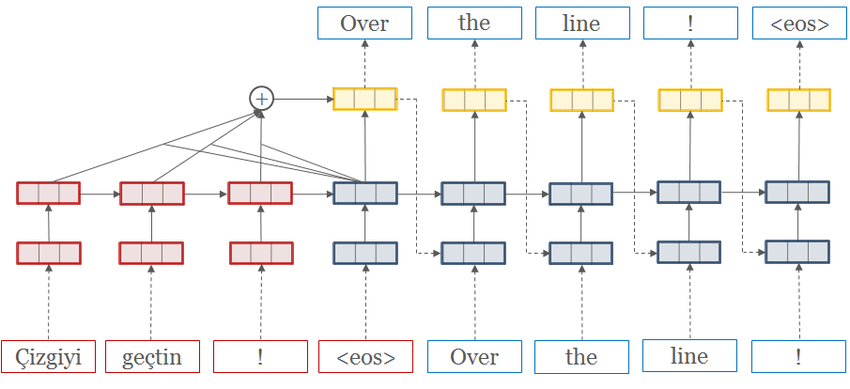
\includegraphics[width=\textwidth]{figures/openmt.png}
\caption{ Schematic view of neural machine translation implemented in OpenNMT\citep{opennmt}.  } \label{fig1}
\end{figure}


\subsubsection{System Efficiency}

One of the biggest concerns about the Neural Machine Translation Systems is the training efficiency, the systems take huge time to train sometimes ranging from days to weeks. The authors tried to address the issue and tried to make the training slightly faster in OpenNMT. 

\textbf{Memory Sharing} The most common reason for high time consumption while training GPU-based NMT models is due to the memory size restrictions which limit the batch size. Though neural network toolkits like Torch has been designed to trade-off the surplus memory allocations for speed and declarative simplicity. For OpenNMT they implemented an external memory sharing system that utilizes the time-series control flow of NMT systems and vigorously shares the internal buffers between the clones. This implementation of vigorously memory reuse results in conservation of about 70\% of GPU memory with the default model size.

\textbf{Multi-GPU} The authors added support for multi-GPU training using data parallelism. Two modes were made available: synchronous and asynchronous training. In synchronous training, the batches run concurrently on parallel GPU and gradients aggregated to update master parameters before resynchronization on each GPU for the next batch. While in asynchronous training, the batches run independent on each GPU and independent gradients accumulated to the master copy of the parameters. Asynchronous SGD is known to provide faster convergence \citep{NIPS2012_4687}. 

\textbf{C/Mobile/GPU Translation} The authors included several different translation models for different run-time environments in OpenNMT: a batched CPU/GPU implementation for quick translation of large set of sentences, a simple single-instance implementation for use on mobile devices and a specialized C implementation. 

\subsubsection{Modularity for Research}

The secondary goal for the authors were to make the code readable for non-experts and they targeted this goal by explicitly separating out optimizations from the core model and by including tutorial documentations within the code. 


\subsubsection{Extensibility}

The field of Deep Learning is quickly evolving and technologies change very frequently. The authors went to perform different case studies to ensure that OpenNMT adhere to code extensibility and support the future variants.

Table \ref{opentable} shows the performance results of OpenNMT against Neamtus , which shows the performance of OpenNMT models were much better than Nematus. Both the systems were having 2x500 RNN, embedding,size of 300, trained for 13 epochs, batch size of 64 and beam size of 5.


\begin{table}[h!]
\caption{Performance Results for EN→DE on WMT15
tested on newstest2014.\citep{opennmt}\label{long}}
\centering
 \begin{tabular}{ |c|c|c|c|c| } 
 \hline Vocab & System & Speed Train & tok/sec Trans & BLEU \\ 
 \hline V=50K & Nematus & 3393 & 284 & 17.28 
 &&OpenNMT&4185&380&17.60\\ 
  \hline V=32K & Nematus & 3221 & 252 & 18.25 
 &&OpenNMT & 5254 & 457 & 19.34\\ 
 \hline
 \end{tabular}
 \label{opentable}
\end{table}

\subsection{Nematus}

Nematus is an open source toolkit developed by \cite{DBLP:journals/corr/SennrichFCBHHJL17} from the Edinburgh NLP group\footnote{\url{http:/edinburghnlp.inf.ed.ac.uk/}, accessed:15.08.2018}, it is implemented in Python and based on the Theano framework \citep{DBLP:journals/corr/Al-RfouAAa16} . They implemented an attentional encoder-decoder architecture which is similar to the one described by \cite{DBLP:journals/corr/BahdanauCB14} , but there were several implementational differences.
\begin{itemize}
\item In the implementation of Nematus they initialized the decoder hidden state with the mean of the source annotation, rather than the annotation at the last position of the encoder backward RNN. 
\item They implemented a new conditional GRU with attention for Nematus.
\item In the decoder, they used a feedforward hidden layer with tanh non-linearity rather than a maxout before the softmax layer.
\item They didn’t implement any additional biases for both encoder and decoder embedding layers.
\item The implementation of \cite{DBLP:journals/corr/BahdanauCB14} used Look, Generate, Update decoder phases whereas in Nematus they implemented Look, Update, Generate which simplified decoder implementation significantly (See Table 1). 
\item They performed recurrent Bayesian dropout \citep{Gal:2016:TGA:3157096.3157211}.
\item In Nematus they allowed multiple features (or “factors”) at each time step instead of a single word embedding at each source position, with the final embedding being the concatenation of the embeddings of each feature \citep{DBLP:journals/corr/SennrichH16}.
\item They allowed tying of embedding matrices \citep{DBLP:journals/corr/PressW16,DBLP:journals/corr/InanKS16}.
\end{itemize}

\begin{table}[h!]
\centering
 \begin{tabular}{ |ll|ll|} 
 \hline
 \multicolumn{2}{|l|}{RNNSearch \citep{DBLP:journals/corr/BahdanauCB14}} & \multicolumn{2}{l|}{Nematus (DL4MT)}\\
  \hline  Phase & Output - Input & Phase & Output - Input \\
  \hline Look & $C_j$ $\leftarrow$ $S_{j-1}$ ,C & Look & $C_j$ $\leftarrow$ $S_{j-1}$, $Y_{j-1}$ ,C \\
  Generate & $Y_j$ $\leftarrow$ $S_{j-1}$, $Y_{j-1}$ ,$C_j$ & Update& $S_j$ $\leftarrow$ $S_{j-1}$, $Y_{j-1}$ ,$C_j$ \\
  Update & $S_j$ $\leftarrow$ $S_{j-1}$, $Y_{j}$ ,$C_j$ & Generate& $Y_j$ $\leftarrow$ $S_{j}$, $Y_{j-1}$ ,$C_j$ \\
  \hline
 \end{tabular}

\caption{Decoder phase differences between Nematus (DL4MT)\citep{DBLP:journals/corr/SennrichFCBHHJL17} and RNNSearch \citep{DBLP:journals/corr/BahdanauCB14}. }
\end{table}

Given a source sequence ($x_1, . . . , x_T_x$ ) of length $T_x$ and a target sequence ($y_1, . . . , y_T_y$ ) of length $T_y$, let $h_i$ be the annotation of the source symbol at position $i$, obtained by concatenating the forward and backward encoder RNN hidden states, $h_i$ = [\overrightarrow{h_i} ; \overleftarrow{h_i} ], and $s_j$ be the decoder hidden state at position $j$.

\textbf{Decoder Initialization} \cite{DBLP:journals/corr/SennrichFCBHHJL17} initialized the decoder hidden state $s$ with the last backward encoder state.
\begin{equation}
S_0 = tanh (W_{init}\overleftarrow{h_i})
\end{equation}

With $W_{init}$ as trained parameters. But in the Nematus implementation they used the average annotation instead:

\begin{equation}
S_0 = tanh (W_{init} \frac{\sum_{i=1}^{T_x}h_i}{T_x})
\end{equation}

\textbf{Conditional GRU with attention} Nematus implemented a novel conditional GRU with attention, $cGRU_{att}$. A $cGRU_{att}$ uses its previous hidden state $s_{j-1}$, the whole set of source annotations $C = {h_1, . . . , h_{T_x}}$ and the previously decoded symbol $y_{j-1}$ in order to update its hidden state $s_j$ , which is further used to decode symbol $y_j$ at position $j$.

\begin{equation}
s_j= cGRU_{att}(s_{j-1},y_{j-1},C)
\end{equation}


The conditional GRU layer with attention mechanism $cGRU_{att}$, consisted of three components : two GRU state transition blocks and an attention mechanism ATT in between. The first transition block, $GRU_1$, combines the previous decoded symbol  $y_{j-1}$ and previous hidden state $s_{j-1}$ in order to generate an intermediate representation $s_j^`$ with the following formulations:


\begin{align*}
s_j^` &= GRU_1(y_{j-1},s_{j-1})=(1-z_j^`)\bigodot \underline{s}_j^`+z_j^`\bigodot s_{j-1}^`,\\
\underline{s}_j^`&= tanh(W^`E[y_{j-1}]+r_j^`\bigodot(U^`s_{j-1})),\\
{r}_j^`&= \sigma (W_r^`E[y_{j-1}]+U_r^`s_{j-1}),\\
{z}_j^`&= \sigma (W_z^`E[y_{j-1}]+U_z^`s_{j-1}),
\end{align*}

, where $E$ is the target word embedding matrix, \underline{s}$_j^`$ is the proposal intermediate representation, $r_j^`$ and $z_j^`$ being the reset and update gate activation. In this formulation, $W^`$ , $U^`$ , $W_r^`$ , $U_r^`$ , $W_z^`$ , $U_z^`$ are trained model parameters; $\sigma$ is the logistic $sigmoid$ activation function \citep{DBLP:journals/corr/SennrichFCBHHJL17}.

In the Nematus implementation, the entire context set $C$ along with intermediate hidden state $s_j$ is taken as input in the attention mechanism ATT, in order to computer the context vector $c_j$ as follows:

\begin{align*}
c_j &= ATT(C,s_j^`)= \sum_{i}^{T_x}{a_{ij}}h_i\\
\alpha_{ij}&= \frac{exp(e_{ij})}{\sum_{k=1}^{T_x}exp(e_{kj})}\\
e_{ij} &= V_{\alpha}^T tanh(U_{\alpha}s_j^`+W__{\alpha}h_i)
\end{align*}
, where $\alpha_{ij}$ is the normalized alignment weight between source symbol at position $i$ and target symbol at position $j$ and $v_\alpha$, $U_\alpha$,$W_\alpha$ are the trained model parameters \citep{DBLP:journals/corr/SennrichFCBHHJL17}.

In the next step , $s_j$ is generated by the second transition block $GRU_2$ 

\begin{align*}
s_j^` = GRU_2(s_j^`,c_j)&=(1-z_j^`)\bigodot \underline{s}_j+z_j\bigodot s_{j}^`,\\
\underline{s}_j&= tanh(Wc_j+r_j\bigodot(Us_j^`)),\\
{r}_j&= \sigma (W_rc_j+U_rs_j^`),\\
{z}_j&= \sigma (W_zc_j+U_zs_j^`),
\end{align*}

, where \underline{s}$_j$ is the proposal hidden state, $r_j$ and $z_j$ being the reset and update gate activation. In this formulation, $W$ , $U$ , $W_r$ , $U_r$ , $W_z$ , $U_z$ are trained model parameters \citep{DBLP:journals/corr/SennrichFCBHHJL17}.

In Nematus, the two implemented GU blocks are not individually recurrent, they are only recurrent at the level of the whole cGRU layer. This way of combining RNN blocks is similar to what is referred in the literature as deep transition RNNs \citep{DBLP:journals/corr/PascanuGCB13,DBLP:journals/corr/ZillySKS16} as opposed to the more common stacked RNNs \citep{doi:10.1162/neco.1992.4.2.234,ElHihi:1995:HRN:2998828.2998898, DBLP:journals/corr/Graves13}.

\textbf{deep output} Given $s_j , y_{j-1},$ and $c_j$ , the output probability $p(y_j|s_j , y_{j-1}, c_j )$ is computed by a softmax activation, using an intermediate representation $t_j$ . 

\begin{align*}
p(y_j|s_j , y_{j-1}, c_j ) = softmax (t_jW_o)\\
t_j=tanh (s_jW_{t1} + E[y_{j-1}]W_{t2} + c_jW_{t3}) \\
\end{align*}

,where $W_{t1},W_{t2},W_{t3},W_o$ are the trained model parameters \citep{DBLP:journals/corr/SennrichFCBHHJL17}.

They designed the Nematus to minimize the cross-entropy on parallel training corpus. For the training they used stochastic gradient descent, or one of its variants with adaptive learning rate Adadelta \citep{DBLP:journals/corr/abs-1212-5701}, RmsProp\citep{hinton} , Adam \citep{DBLP:journals/corr/KingmaB14}. Further, to optimize towards arbitrary, sentence level loss function they provided support for minimum risk training (MRT) \citep{DBLP:journals/corr/ShenCHHWSL15}. 

\begin{figure}
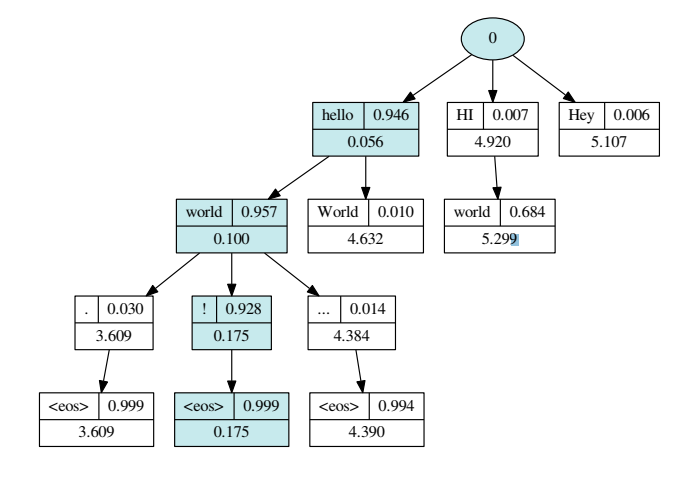
\includegraphics[width=\textwidth,height=250pt]{figures/nematus.png}
\caption{ Search graph visualisation for DE$\rightarrow$ EN
translation of "Hallo Welt!" with beam size 3 using Nematus\citep{DBLP:journals/corr/SennrichFCBHHJL17}.} \label{fignm2}
\end{figure}

\subsection{Neural Monkey}
Neural Monkey is an open-source toolkit written using the TensorFlow machine learning library \citep{DBLP:journals/corr/AbadiABBCCCDDDG16} developed by \cite{neuralmonk}. It provides a higher level API, such that it should be enough for the users to be familiar with the models on the equation level, without delving into implementation details. As compared to other open-source NMT toolkits, Neural Monkey provides a higher level of abstraction, along with a simple configuration mechanism that allows for fast prototyping and reusing trained models and experiment management.

The building blocks of Neural Monkey are not individual network layers like \textit{tfLearn}\footnote{\url{http://tflearn.org/},accessed:11.08.2018} or \textit{Lasagne}\footnote{\url{https://github.com/Lasagne/Lasagne/},accessed:11.08.2018} , but they are more abstract objects like encoders and classifiers. These objects are parametrized so that their properties (e.g. number and sizes of hidden layers or dropout probability) can be set from a farther perspective \citep{neuralmonk}. This design process allowed the authors to separate the configuration of the experiments from the actual code, which prevented the users from interleaving the configuration with other program logic. 

\begin{figure}
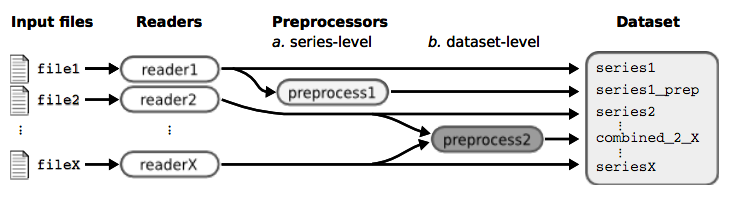
\includegraphics[width=\textwidth]{figures/nmonkey2.png}
\caption{ Creation of Dataset in Neural Monkey \citep{neuralmonk}.} \label{fignm2}
\end{figure}

In Neural Translation Systems, the loading and processing of datasets is one of the most important systems. The dataset in Neural Monkey is created in three step, first an input file is read using a Reader which load a file containing paths to JPEG images and load them as NumPy arrays, or read tokenized text as a list of lists of string tokens. The next phase is pre-processors, the series created by the readers is pre-processed by the system such as byte-pair encoding \citep{P16-1162} which loads a list of merges and segments the text accordingly. Finally, the dataset-level pre-processors are applied of multiple series data to create the final dataset. 

\begin{figure}
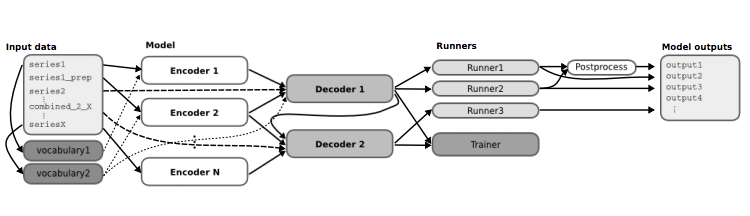
\includegraphics[width=\textwidth]{figures/nmonkey1.png}
\caption{ Model workflow in Neural Monkey \citep{neuralmonk}} \label{fignm1}
\end{figure}


The model in Neural Monkey is defined by different model parts such as encoders and decoders. The authors defined the encoders and decoders in more general than the classical Sequence to Sequence Learning. They defined the Encoders as parts of the model which take the input and compute a representation of it. They used runners for the execution of the Decoders. They designed different runners to represent different ways of running the model. They implemented trainer which is a runner to modify the parameters of the model, to collect the objective functions and use them in a optimizer. They used an object called TensorFlow manager to manage all the TensorFlow sessions. 

In order to validate the Neural Monkey’s performance the authors did a sanity check evaluation on the architechture introduced by \cite{DBLP:journals/corr/BahdanauCB14} which became the standard baseline model in NMT research. 


They used a bi-directional GRU network with 500 hidden units in each direction as the encoder and for decoder they used an RNN decoder with 1000 units in the hidden layer. They used a simple ‘tanh’ projection instead of max-out projection as used in the original model. The original paper used Adadelta \citep {DBLP:journals/corr/abs-1212-5701} optimizer, whereas for this comparative study they used Adam \citep{DBLP:journals/corr/KingmaB14} . The comparison of the models is shown in Table \ref{neumonk}. 

\begin{table}[h!]
\centering
 \begin{tabular}{ |c|c|c| } 
  \hline Model & BLEU & epoch \\ 
  \hline  \cite{DBLP:journals/corr/BahdanauCB14} - neural & 26.75 & 2.2\\
 \cite{DBLP:journals/corr/BahdanauCB14} - neural & 28.45 & 6.0\\
  SMT & 33.30 & -\\
  \hline Neural Monkey - greedy decoding & 25.08 & 1.2\\
  Neural Monkey + CGRU – greedy decoding  & 27.35 & 1.6\\
  \hline
 \end{tabular}
\caption{Results achieved by Neural Monkey on the WMT14 News Task French to English dataset with the number epochs \citep{neuralmonk}.}
\label{neumonk}
\end{table}

\section{Related Work}

In WAT 2017\footnote{{\url{http://lotus.kuee.kyoto-u.ac.jp/WAT/WAT2017/},accessed:20.08.2018}} , the convolutional sequence to sequence model by  \cite{Singh2017ComparingRA} achieved a BLEU score 12.23 for English to Hindi translations using the same corpus. In the same workshop, the baseline system designed by \cite{W17-5707} achieved a BLEU score of 13.69. 


\cite{Revanuru:2017:NMT:3140107.3140111} created a system with multiple models which were used for six Indian language pairs. The compared the results of their system with Google Translate, and their best model outperformed Google Translate by a margin of 17 BLEU points on Urdu-Hindi, 29 BLEU points on Punjabi-Hindi, and 30 BLEU points on Gujarati-Hindi translations.

\cite{10.1007/978-3-319-63645-0_55} created a translation tool named English to Hindi Translator using Translation Memory which can transform an English sentence to its proper Hindi meaning. This translator works on both exact match and fuzzy match. 

\cite{10.1007/978-981-10-8657-1_62} created an Indic machine translation system that utilized recent advancement in the area of machine translation using deep neural architectures. The results showed that neural machine translation systems can yield more natural translations than rule based or phrase based translation systems.

\section{Conclusion}

In this chapter, the background and State of the Art were discussed, in order to address the research question. The previous researches field of machine translation were presented with the focus on concepts and principles centered on this research pursuit.

Next, the previous works in the field of Statistical Machine Translation was introduced and formally discussed. The evolution of Statistical Machine Translation from Word Based Models to Phrase based models were discussed in depth as it paves the base of this research.

Finally, research within the area of Neural Machine Translation was discussed, focusing on the time-line of historical research and the latest innovations in the study of machine translations. Google's state of art neural machine translation was discussed in details as it is a major motivation for this research. These are studies that closely relate to this work in their concerns and aims.

In concluding the State of the Art, the related works in the area of neural machine translations in English-Hindi  is discussed. There appears a substantial gap in the area of neural machine translation in Hindi-English. 

The goal of this work is to use neural machine translation on a larger Hindi-English corpora and produce above average translations which are more generic. And subsequently, fine tuning the trained model using a new domain specific smaller corpus to produce better domain specific results.  

  \chapter{Design and Methodology}
\section{Data Gathering}
\section{Neural Translation Model}
\section{Visual Interface}
  \chapter{Implementation}
\section{Data Gathering}
\subsection{Training Dataset}
\subsubsection{TED Talks}
\begin{figure}
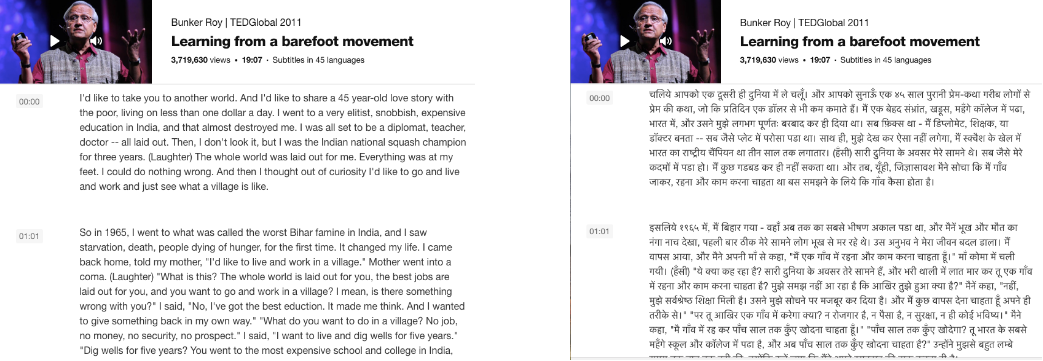
\includegraphics[width=\textwidth]{figures/tedtalks.png}
\caption{A side-by-side figure showing TED Talk transcripts in English and Hindi} \label{fig1}
\end{figure}
\subsubsection{Beautiful Soup}
Beautiful Soup is one of the most widely used open source Python library designed by Leonard Richardson for quick turnaround projects like website scrapping. The decision to use Beautiful Soup for this research was motivated by the fact that It provides simple methods and Pythonic idioms for navigating, searching and modifying a parse tree. It’s a simple toolkit for dissecting the document and extracting the relevant information according to the user’s need. Beautiful Soup makes the handling of encodings much easier, it automatically converts incoming documents to Unicode and outgoing documents to UTF-8. The library sits on top of Popular parsers like lxml and html5lib which allows the user to try different parsing strategies or trade speed for flexibility. 
\subsubsection{Indic NLP Library}
Indic NLP Library is an open source Python Based Library for common text processing and Natural Language Processing in Indian Languages developed by Anoop Kunchukuttan.  The Indian Languages are originated from Sanskrit and are quite different from the Latin-Based Languages or other Asian Languages, so the other NLP Libraries doesn’t perform well on Indian Languages. Though the Indian languages share a lot of similarity among themselves in terms of script, phonology, language syntax, etc. There are very few researches going in the field of Hindi NLP, and Indic NLP Library is the only existing NLP library for the Hindi language. The library provides several functionalities such as Text Normalization, Tokenization, and Morphological Analysis.
\subsubsection{Moses Tokenizer}
Moses is one of the most successful implementations of the Statistical Machine Translation which was the dominant approach before the onset of Neural Machine Translation. Moses provides several tools for Statistical Machine Translation process, such as for Corpus preparation it provides tokenization, true casing and cleaning tools. As the process of preparation of corpus remains same for Neural Machine Translation Systems, the Moses Tokenizer was chosen here for the tokenization of the English text. 
\subsubsection{TED Hindi English Corpus}
\begin{figure}
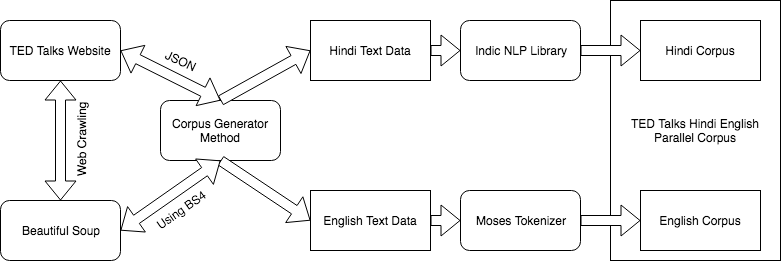
\includegraphics[width=\textwidth]{figures/traindataworkflow.png}
\caption{Workflow of the TED Talks Corpus Generator} \label{fig1}
\end{figure}
TED.com discontinued their Open API project and so there is no direct way to fetch the transcripts of talks. TED.com is a static website, so talks link location is static and can be accessed if prior information of talks details is obtained through Beautiful soup and $urllib$ library in python 

Firstly, the Beautiful Soup library is used to fetch the links of all the 396 TED Talks which are available in the Hindi language from the home page of the TED Official Website. The URL of the web page is passed to the method which implements the Beautiful Soup.  For each and every web page, the $find/_$all() method finds all the “$a$” tags in the respective pages. Further, $attrs$ method is used to find all the $“href”$ which are having "$/talks$". The URL to the original talks is obtained and stored in a list for further parsing. The method is iterated through the entire list of pages having Hindi TED Talks. 

The transcripts for the talks are fetched from TED’s internal server which is having an open access and URL is appended "$transcript.json?language=en$" . Two different methods for English and Hindi are implemented to obtain the JSON from the respective URLs and load into the data file. 

The JSON is parsed by the respective methods and the transcript text is obtained. The JSON data consisted of time frames, translated text of available language which here Hindi and English respectively. The methods parse the JSON data, fetch the translation and write it in two separate text files “$Hindi.txt$” and “$English.txt$” to create the Hindi-English Parallel Corpus.

The text files generated by the methods were ill-formatted and contained junk texts. So, there was a need for Normalization and Tokenization of the text files. The text written in Hindi displays a lot of quirky behavior on varying input or multiple representations of the same character, so there was a need to canonicalize the representation of the text such that the NLP applications can handle the data inconsistent manner. The canonicalization of the text files handled issues such as,
\begin{itemize}
\item Non-Spacing characters like ZWJ/ZWNL
\item Multiple Representations of Nukta based Characters
\item Multiple Representations of two-part dependent vowel signs
\item Typing inconsistencies: e.g. use of pipe ($|$) for poorna virama 
\end{itemize}

Further the tokenizer in the library was used to tokenize the Hindi text and make it ready for corpora.

The Moses tokenizer comes with two perl scripts which takes two

\subsection{Test Data}
\subsubsection{Blog Content from Tripoto}
\subsubsection{Sumy}
Sumy is an Open Source python library and python command line utility for extracting a summary from HTML pages or plain texts, developed by Miso Belica. The package also contains a simple evaluation framework for text summaries.The decision to use sumy was driven by a number of factors.Sumy is an extractive text summarizer.Extractive text summarization techniques perform summarization by extracting portions of texts and constructing a summary, while the abstractive techniques like Google's TextSum learn the internal language representation to generate more human-like summaries,
and paraphrases the original text. Extractive text summarization makes more sense in the summarization of Blogs as it keeps the original text which highlights the author’s point of view and writing style. Secondly, the abstractive text summarization is technique is highly unfeasible considering the available infrastructure at this stage of research.Further, Sumy provides seven different summarization methods which gives a choice to choose the best summarization algorithm for the blog summarization. 

The methods are as follows: 

\begin{itemize}
    \item Luhn is one of the earliest suggested algorithms by the famous IBM researcher it was named after and it scores sentences based on the frequency of the most important words. The algorithm derives statistical information from word frequency and distribution to compute a relative measure of significance. The sentence which scores relatively higher than others is extracted to create a summary. 
    \item Edmundson is a heuristic method which implements previous statistic research of high-frequency words along with the three additional components: pragmatic words (cue words); title and heading words; and structural indicators (sentence location). 
    
\end{itemize}

\subsubsection{Summarizer}

\begin{figure}
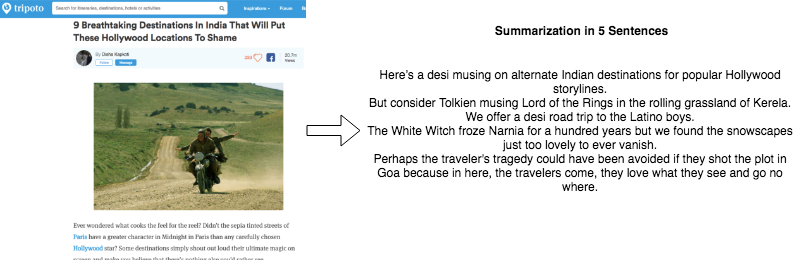
\includegraphics[width=\textwidth]{figures/textsummary.png}
\caption{Histogram of side-by-side scores on 500 sampled sentences from Wikipedia and news websites for a
typical language pair, here English to Spanish (PBMT blue, GNMT red, Human orange). It can be seen that
there is a wide distribution in scores, even for the human translation when rated by other humans, which
shows how ambiguous the task is. It is clear that GNMT is much more accurate than PBMT.} \label{fig1}
\end{figure}
Tripoto is one of the biggest Travel Blogging Websites in the World. The method implements the Beautiful Soup library and fetches the list of 50 most popular blogs from the URL “$https://www.tripoto.com/trips$ “. The links to the respective blogs is written into a csv (comma separated values) file for the summarization.

The method which implements the sumy library reads the csv file and creates a 5-sentence summary for each and every blog. After experimenting with LexRank, TextRank and Latent Semantic Analysis (LSA), LSA is finally used as the summarizer based on the quality of the summary. The Summary is then saved in a csv file corresponding to their blog links, which is further used by the Visual Interface. 

\section{Neural Translation Model}
\subsection{Keras}
Keras is an open source high-level neural networks API, which is written in Python and capable of running on top of TensorFlow, CNTK, and Theano.  It was designed to enable fast experimentation with deep neural networks and make neural network programming more user-friendly, modular and extensible. The decision to use Keras was driven by a number of factors. Firstly, Keras allows for easy and fast prototyping with minimal lines of code, it’s easier to code than TensorFlow.  In Keras, a model is represented as a sequence or a graph of standalone, fully-configurable modules that can be linked together with very limited restrictions. The neural layers, cost functions, optimizers, activation functions, regularization schemes are all standalone modules that can be combined easily to create new models. 
\subsection{Seq2Seq Model}
\section{Visual Interface}

  \chapter{Evaluation}
\section{Approach}
\section{BLEU}
\section{Human Evaluation}
\section{Discussion}
  \chapter{Conclusion}
\section{Data Gathering}

Random citation \cite{sterner2002ecological} embed deed in text.

\begin{thebibliography}{ieeetr}                   %% Start your bibliography here; you can
\bibliography{refs.bib}                               %% also use the \bibliography command
\end{thebibliography}                             %% to generate your bibliography.


\addcontentsline {toc}{chapter}{Appendices}       %% Force Appendices to appear in contents
\begin{appendix}
 \chapter*{Appendix}

...

% \include{appendix2}
\end{appendix}


%\addcontentsline {toc}{chapter}{Bibliography}     %% Force Bibliography to appear in contents


\end{document}                                    %% END THE DOCUMENT
